\documentclass[11pt,a4paper]{article}

\usepackage[T1]{fontenc}
\usepackage[utf8]{inputenc}
\usepackage[spanish,es-tabla,es-noshorthands]{babel}
\usepackage{lmodern}
\usepackage[margin=2.5cm]{geometry}
\usepackage{graphicx}
\usepackage{booktabs}
\usepackage{multirow}
\usepackage{array}
\usepackage{caption}
\usepackage{float}
\usepackage{csquotes}
\usepackage[style=authoryear,maxcitenames=2,maxbibnames=6,backend=biber]{biblatex}
\usepackage[hidelinks]{hyperref}

\addbibresource{referencias.bib}
\graphicspath{{../results/figures/}}

\newcommand{\cod}[1]{\texttt{#1}}

\title{Entender quien escribe mal:\\
  robustez de clasificadores de intenciones en español\\
  frente a ruido de escritura}
\author{Grupo 1 --- Benitez, Tomás; Lombardia, Maximiliano;\\
  Mónaco, Vianca; Vollert, Marcos}
\date{Universidad de Palermo --- Procesamiento de Lenguaje Natural --- 4/11/2026}

\begin{document}

\maketitle

\begin{abstract}
Los asistentes virtuales se entrenan con frases bien escritas, pero en producción reciben
texto sin tildes, con errores de tipeo, abreviado o con expresiones regionales. Este trabajo
estudia cuánto se degradan cinco clasificadores de intenciones en español ante ese ruido, y si
las representaciones basadas en subpalabras resisten mejor que las basadas en palabras
completas. Sobre el corpus MASSIVE (es-ES, 60 intenciones) se compararon TF-IDF de palabras y
de caracteres con regresión logística, FastText con y sin subpalabras, y BETO ajustado por
fine-tuning, frente a siete perturbaciones sintéticas en cinco intensidades. Con errores de
tipeo la hipótesis se confirma: el mismo modelo FastText se degrada mucho menos cuando usa
subpalabras. Sin embargo, BETO, que también usa subpalabras, es el mejor modelo sin ruido pero
cae casi tanto como los modelos de palabras con typos intensos, mientras que TF-IDF de
caracteres es el más robusto. Ante cambios de vocabulario y voseo, en cambio, BETO es el que
menos se degrada. Como complemento, dos LLM locales usados sin entrenamiento no superaron a
TF-IDF de caracteres en ninguna condición y fueron mucho más lentos.
\end{abstract}

% ---------------------------------------------------------------------------
\section{Introducción}

Un clasificador de intenciones decide qué quiere hacer el usuario de un asistente virtual
(poner una alarma, consultar el clima, reproducir música) a
partir de una frase. Los corpus con los que se entrenan estos sistemas suelen estar escritos
con cuidado, pero los usuarios reales escriben rápido y de forma informal: omiten tildes,
cometen errores de tipeo, abrevian o usan vocabulario y
conjugaciones propias de su región. Un modelo con buen rendimiento en el conjunto de evaluación puede degradarse
fuertemente ante esas variaciones.

La forma en que el modelo representa el texto debería influir en esa degradación. Un modelo que
solo conoce palabras completas trata \enquote{alarma} y \enquote{slarma} como dos símbolos sin
relación: el segundo nunca apareció en el entrenamiento y se ignora. Un modelo que mira
fragmentos de la palabra (\enquote{lar}, \enquote{arm}, \enquote{rma}) todavía reconoce la
mayoría de ellos en la forma mal escrita.

De ahí surge la hipótesis del trabajo:

\begin{quote}
\emph{Las representaciones que incorporan información de subpalabras (n-gramas de caracteres y
tokenizadores de subpalabras de los transformers) son más resistentes a los errores de tipeo
que las representaciones basadas exclusivamente en palabras completas.}
\end{quote}

Como pregunta complementaria, se busca determinar en qué tipos de perturbación se manifiesta
con mayor claridad esa diferencia. Los aportes del trabajo son:
\begin{itemize}
  \item Un conjunto de siete perturbaciones controladas para español, con intensidad graduable,
        deterministas y anidadas entre niveles (\S\ref{sec:perturbaciones}).
  \item Una comparación de cinco clasificadores que incluye un \emph{control experimental}:
        el mismo modelo FastText con y sin subpalabras, que aísla el efecto de la
        representación (\S\ref{sec:modelos}).
  \item Una evaluación con intervalos de confianza por bootstrap pareado sobre frases, que
        distingue diferencias reales de variaciones de muestra (\S\ref{sec:evaluacion}).
  \item Una comparación complementaria con dos LLM locales usados sin entrenamiento, que
        incluye latencia y consumo energético (\S\ref{sec:llm}).
\end{itemize}

% ---------------------------------------------------------------------------
\section{Trabajos relacionados}

\paragraph{Clasificación de texto.} La clasificación de intenciones es un caso de
clasificación de texto corto, una tarea que evolucionó desde los métodos tradicionales, con
representaciones dispersas como TF-IDF sobre modelos de espacio vectorial y clasificadores
lineales como la regresión logística, hasta los embeddings y los modelos profundos
preentrenados. Este trabajo compara representantes de cada etapa de esa evolución sobre la
misma tarea.

\paragraph{De palabras a subpalabras.} En los modelos de espacio vectorial clásicos y en los
embeddings estáticos como word2vec, cada palabra del
vocabulario tiene su propia dimensión o su propio vector. Una palabra que no apareció en el
entrenamiento, como una palabra con un error de tipeo, queda sin representación: es el problema
de las palabras desconocidas. Una respuesta es descomponer las palabras en unidades menores.
FastText, por ejemplo, representa cada palabra como la suma de los vectores de sus n-gramas de
caracteres, y los tokenizadores de subpalabras dividen las palabras poco frecuentes en
fragmentos de un vocabulario fijo.

\paragraph{Transformers y modelos preentrenados.} La arquitectura transformer es la base de
BERT, un codificador preentrenado sobre grandes corpus que luego se ajusta (\emph{fine-tuning})
para cada tarea, como la clasificación de texto, con pocos datos etiquetados. BERT usa un tokenizador de subpalabras, por lo que, en principio, también
debería beneficiarse de la descomposición de palabras desconocidas.

\paragraph{LLM como clasificadores.} Los modelos de lenguaje grandes pueden resolver tareas sin
ajustar sus pesos: sin ejemplos, a partir de una instrucción, o con unos pocos ejemplos en el
prompt (\emph{few-shot}). Esa capacidad mejora con la escala del modelo, pero también crecen su
costo computacional y energético. Por eso tiene sentido
preguntarse si un LLM chico, ejecutado localmente, es una alternativa competitiva a un
clasificador entrenado.

\paragraph{Lo que aborda este trabajo.} La bibliografía revisada explica por qué las
subpalabras deberían ayudar ante palabras desconocidas, pero no cuantifica cuánto ayudan ante
cada tipo de ruido de escritura ni si todos los esquemas de subpalabras se comportan igual.
Este trabajo lo mide experimentalmente, en español y para clasificación de intenciones, con
ruido de intensidad controlada.

% ---------------------------------------------------------------------------
\section{Metodología}

\subsection{Datos}

Se usó MASSIVE, un corpus de comprensión del lenguaje para asistentes virtuales publicado por
Amazon Science, con alrededor de un millón de frases en 51 idiomas.\footnote{\url{https://github.com/alexa/massive}}
Se trabajó con la partición es-ES, que contiene frases cortas con 60 intenciones (por ejemplo
\cod{alarm\_set}, \cod{play\_music}, \cod{weather\_query}). Los tamaños son 11\,514 frases de entrenamiento, 2\,033 de validación
y 2\,974 de test. Los datos se cargaron desde la réplica \cod{mteb/amazon\_massive\_intent} de
Hugging Face, con una revisión fija, porque el repositorio original usa un script de carga que
las versiones actuales de la biblioteca \cod{datasets} ya no admiten. Se verificó que textos,
etiquetas e identificadores coinciden con el parquet oficial en los tres conjuntos.

\paragraph{Uso de los conjuntos.} Siguiendo la propuesta, \textbf{train} se usó para entrenar,
\textbf{test} para elegir hiperparámetros y \textbf{validation} para la evaluación final, tanto
sin ruido como con ruido. Es la convención inversa a la habitual, pero metodológicamente
equivalente: los dos conjuntos provienen de la misma distribución y lo importante es que la
robustez se mida sobre frases que no intervinieron en la selección de hiperparámetros. Por eso
todo el rendimiento se reporta sobre validation.

\paragraph{Características relevantes.} Las frases de MASSIVE ya vienen en minúsculas y casi
sin puntuación (solo el 1,5~\% tiene algún signo). Validation no contiene la intención
\cod{audio\_volume\_other}, por lo que tiene 59 intenciones, y seis de ellas tienen cinco frases
o menos.

\subsection{Modelos}
\label{sec:modelos}

Se entrenaron cinco clasificadores, agrupados según cómo representan el texto
(Tabla~\ref{tab:modelos}). Los hiperparámetros de TF-IDF y FastText se eligieron con búsquedas
pequeñas sobre test.

\begin{table}[H]
\centering
\small
\begin{tabular}{@{}l p{8.2cm} l@{}}
\toprule
Modelo & Representación y clasificador & Grupo \\
\midrule
TF-IDF palabras & TF-IDF de 1 y 2-gramas de palabras + regresión logística & Palabras \\
TF-IDF caracteres & TF-IDF de n-gramas de caracteres (2 a 5) dentro de cada palabra +
  regresión logística & Subpalabras \\
FastText sin subpalabras & FastText supervisado, solo palabras y bigramas & Palabras \\
FastText con subpalabras & FastText supervisado con n-gramas de caracteres de 3 a 6 &
  Subpalabras \\
BETO & Fine-tuning de BERT preentrenado en español, con tokenizador WordPiece & Subpalabras \\
\bottomrule
\end{tabular}
\caption{Modelos comparados.}
\label{tab:modelos}
\end{table}

\paragraph{TF-IDF y regresión logística.} Cada frase se representa como un vector disperso
ponderado por TF-IDF, con frecuencia sublineal
($1+\log \mathrm{tf}$). La variante de caracteres usa n-gramas que no cruzan los espacios entre
palabras. Sobre ese vector se entrena una regresión logística multiclase
con $C=10$ (se probaron 1, 10 y 30). Se implementó con
scikit-learn.

\paragraph{FastText.} Aprende un embedding de 100 dimensiones por palabra, promedia los de la
frase y clasifica con una capa lineal (\cod{lr}~=~0,5, 100 épocas, bigramas de palabras). Con
subpalabras, el vector de cada palabra es la suma de los vectores de sus n-gramas de 3 a 6
caracteres, de modo que una palabra mal escrita recibe un vector cercano al de la original.
La variante sin subpalabras usa exactamente los mismos hiperparámetros y es el control
experimental del trabajo: si la versión con subpalabras resiste más, la diferencia se debe
solo a la representación. Como FastText~0.9.2 no es determinista dentro de un mismo proceso,
cada entrenamiento se hace en un proceso nuevo.

\paragraph{BETO.} BETO es un modelo BERT preentrenado en español
por la Universidad de Chile. Se partió de su versión
\cod{dccuchile/bert-base-spanish-wwm-cased},\footnote{\url{https://huggingface.co/dccuchile/bert-base-spanish-wwm-cased}}
se le agregó una capa de clasificación y se ajustó durante 3 épocas (tasa de aprendizaje
$5\times10^{-5}$, lote de 32, \emph{weight decay} de 0,01, \emph{warmup} del 10~\%, máximo de
64 tokens) con la biblioteca Hugging Face Transformers, siguiendo el procedimiento habitual de
clasificación con transformers. Su tokenizador
WordPiece deja las palabras frecuentes enteras
y parte las raras o mal escritas en fragmentos: \enquote{alarma} es un único token, pero
\enquote{slarma} se divide en \enquote{s}, \enquote{lar} y \enquote{ma}. Por eso
cuenta como modelo de subpalabras, aunque con un vocabulario fijo.

\paragraph{Semillas de entrenamiento.} FastText y BETO se entrenaron con tres semillas (42 a
44) y se promediaron. La regresión logística con el solver \emph{lbfgs} produce el mismo modelo
con cualquier semilla, así que TF-IDF se entrenó una sola vez.

\subsection{Perturbaciones}
\label{sec:perturbaciones}

Se diseñaron siete perturbaciones que modelan fenómenos frecuentes en la escritura informal
(Tabla~\ref{tab:perturbaciones}). Cada una tiene una intensidad $p \in [0,1]$ y se evaluó en
$p \in \{0{,}1;\ 0{,}25;\ 0{,}5;\ 0{,}75;\ 1{,}0\}$.

\begin{table}[H]
\centering
\small
\begin{tabular}{@{}l p{6.6cm} p{4.2cm}@{}}
\toprule
Perturbación & Qué hace & Cómo actúa $p$ \\
\midrule
Sin tildes & \enquote{canción} $\to$ \enquote{cancion} (conserva la ñ) &
  probabilidad por carácter acentuado \\
Minúsculas y sin puntuación & elimina mayúsculas y los signos \cod{.,¿?¡!} &
  probabilidad por frase \\
Errores de tipeo & tecla vecina en un teclado QWERTY español, letra borrada, duplicada o dos
  letras intercambiadas & probabilidad por palabra de 3 letras o más \\
Abreviaturas & \enquote{por favor} $\to$ \enquote{xfa}, \enquote{que} $\to$ \enquote{q},
  \enquote{para} $\to$ \enquote{pa}, \enquote{cinco} $\to$ \enquote{5} (32 entradas) &
  probabilidad por ocurrencia \\
Voseo rioplatense & \enquote{pon} $\to$ \enquote{poné}, \enquote{dime} $\to$
  \enquote{decime}, \enquote{enciende} $\to$ \enquote{prendé} (16 entradas) &
  probabilidad por ocurrencia \\
Vocabulario coloquial & \enquote{correo electrónico} $\to$ \enquote{mail}, \enquote{canción}
  $\to$ \enquote{tema}, \enquote{necesito} $\to$ \enquote{me hace falta} (18 entradas) &
  probabilidad por ocurrencia \\
Combinado & todas en cadena: coloquial, voseo, abreviaturas, minúsculas, tildes y typos &
  la misma $p$ para todas \\
\bottomrule
\end{tabular}
\caption{Perturbaciones aplicadas sobre validation.}
\label{tab:perturbaciones}
\end{table}

\paragraph{Diseño.} Cada unidad de la frase (palabra, carácter acentuado u ocurrencia de una
entrada del diccionario) tiene su propio generador aleatorio, que depende de la semilla, de la
perturbación, del texto y de la posición, pero no de $p$ ni de las demás frases. Esto garantiza
tres propiedades, verificadas con tests automáticos: el mismo conjunto se genera idéntico cada
vez; una frase recibe el mismo ruido sola o dentro de un lote; y los niveles son
\emph{anidados}, es decir, lo que se altera con $p=0{,}1$ sigue alterado igual con $p=0{,}25$.
Así, entre un nivel y el siguiente solo se agregan errores, y las curvas de degradación no
mezclan el efecto de la intensidad con el azar de qué palabras se eligieron. En los typos,
primero se elige la operación, de forma equiprobable, y luego una posición donde esa operación
efectivamente modifique la palabra.

\paragraph{Diccionarios.} Los diccionarios de abreviaturas, voseo y vocabulario coloquial se
armaron a mano. Cada reemplazo se revisó sobre los contextos en que la palabra aparece en
\emph{train}, no en validation ni en test, para no diseñar el ruido mirando el conjunto de
evaluación. Se descartaron reemplazos que cambiaban el significado en el corpus: por ejemplo,
\enquote{vale} $\to$ \enquote{dale} (en MASSIVE es el verbo \emph{valer}), \enquote{móvil}
$\to$ \enquote{celu} (aparece como adjetivo en \enquote{media móvil}) o \enquote{uno} $\to$
\enquote{1} (casi siempre es pronombre). El voseo y el vocabulario se separaron porque son
fenómenos distintos: el primero cambia la morfología del verbo y conserva gran parte de la
forma escrita, mientras que el segundo reemplaza una palabra por otra sin relación
ortográfica. En la perturbación combinada los diccionarios se aplican antes que los typos,
porque buscan palabras bien escritas.

\paragraph{Semillas de ruido.} Cada perturbación se generó con cinco semillas (42 a 46). En
total se evaluaron 176 conjuntos de validation: el limpio más 7 perturbaciones $\times$ 5
intensidades $\times$ 5 semillas. La Tabla~\ref{tab:ejemplos} muestra ejemplos reales.

\begin{table}[H]
\centering
\small
\begin{tabular}{@{}l l@{}}
\toprule
Perturbación ($p$) & Frase \\
\midrule
Original & envía un correo electrónico a mi jefe diciendo que llego tarde \\
Sin tildes (1,0) & envia un correo electronico a mi jefe diciendo que llego tarde \\
Errores de tipeo (1,0) & ejvía un corrreo electróinco a mi jfe diciedno \ldots \\
Voseo (1,0) & mandá un correo electrónico a mi jefe diciendo \ldots \\
Coloquial (1,0) & envía un mail a mi jefe diciendo que llego tarde \\
Combinado (1,0) & mqnda un maiil a mi jfee diciedno q lleggo tarse \\
\midrule
Original & ponme una alarma para mañana a las siete por favor \\
Abreviaturas (0,5) & ponme una alarma pa mñn a las 7 xfa \\
Voseo (0,5) & poneme una alarma para mañana a las siete por \ldots \\
\bottomrule
\end{tabular}
\caption{Ejemplos de perturbaciones generadas.}
\label{tab:ejemplos}
\end{table}

\subsection{Evaluación}
\label{sec:evaluacion}

\paragraph{Métricas.} Se reportan accuracy y F1 macro. El F1 macro promedia el F1 de cada
intención sin ponderar por frecuencia, de modo que penaliza fallar en intenciones poco
frecuentes. Se promedia solo sobre las intenciones presentes en el conjunto (59 en
validation): si se incluyeran las intenciones predichas que no están en el conjunto, cada una
sumaría un F1 de 0 y el promedio dejaría de ser comparable entre modelos y niveles de ruido.

\paragraph{Caída de rendimiento.} Los modelos no rinden igual sin ruido, por lo que la robustez
se compara mediante la \emph{caída}: la accuracy limpia menos la accuracy con ruido, en puntos
absolutos, calculada sobre las mismas frases. Esto también es necesario porque sin ruido los
modelos ya se equivocan en el 13 al 21~\% de las frases: con typos a $p=0{,}25$, entre el 52 y
el 75~\% de los errores ya existían en la versión limpia.

\paragraph{Intervalos de confianza.} La caída se acompaña de un intervalo de confianza del
95~\% obtenido por \emph{bootstrap pareado}:
se remuestrean frases con reposición (1\,000 remuestreos) y cada frase aporta juntas su versión
limpia y sus versiones con ruido, promediadas sobre semillas. Para comparar dos modelos se
calcula, del mismo modo, la diferencia entre sus caídas; si el intervalo no incluye el 0, la
diferencia no se explica por la muestra de frases. Se usa accuracy porque se descompone por
frase, lo que no ocurre con el F1 macro. Estos intervalos no incluyen la variabilidad entre
semillas de entrenamiento, que se informa por separado.

\subsection{Comparación complementaria con LLM locales}
\label{sec:llm-metodo}

Se agregó una comparación opcional con LLM chicos
ejecutados localmente mediante Ollama:\footnote{\url{https://ollama.com}} \cod{llama3.1} (8B
parámetros, de Meta) y \cod{qwen3.5:4b} (4B parámetros, de Alibaba). No se entrenan: el prompt
de sistema contiene las 60 etiquetas y, con $k=2$, dos ejemplos de train por intención, al
estilo \emph{few-shot}. La respuesta se restringe con un esquema JSON a una de las 60 etiquetas,
con temperatura 0 y un contexto de 4\,096 tokens. En \cod{qwen3.5:4b} se desactivó el modo de
razonamiento, porque de lo contrario agota los tokens permitidos y devuelve una respuesta
vacía.

El valor de $k$ se eligió con 500 frases limpias de test, con el mismo criterio que los
hiperparámetros de los demás modelos. \cod{llama3.1} obtuvo 0,572 con $k=0$ y 0,630 con $k=2$;
\cod{qwen3.5:4b}, 0,696 y 0,702. Por su costo, los LLM se evaluaron sobre validation solo con
intensidades 0,25 y 1,0 y con una única semilla de ruido. También se midió la latencia por
frase, el rendimiento en lote y la energía consumida por la GPU.

\subsection{Implementación y reproducibilidad}

El código está en Python. Cada modelo entrenado se guarda con un nombre que incluye un
\emph{hash} de su configuración y de la revisión de los datos, de modo que un cambio de
hiperparámetros obliga a reentrenar en lugar de reutilizar un modelo viejo. Cada ejecución
registra el commit del código, las versiones de las bibliotecas y la plataforma. Los
resultados principales se obtuvieron en una GPU NVIDIA RTX~3080; la corrida completa de los
cinco modelos con todas sus semillas tarda alrededor de cinco minutos.

% ---------------------------------------------------------------------------
\section{Experimentos y resultados}

\subsection{Rendimiento sin ruido}

La Tabla~\ref{tab:limpio} y la Figura~\ref{fig:limpio} muestran el rendimiento sobre
validation sin ruido. BETO es el mejor en accuracy (0,872). En F1 macro, BETO (0,819) y TF-IDF
de caracteres (0,807) quedan dentro de la variabilidad entre semillas de BETO ($\pm$0,014).
En los dos pares de modelos comparables, la versión con subpalabras rinde mejor también sin
ruido.

\begin{table}[H]
\centering
\small
\begin{tabular}{@{}l c c c@{}}
\toprule
Modelo & Accuracy [IC 95~\%] & F1 macro & Semillas \\
\midrule
TF-IDF palabras & 0,813 [0,794; 0,829] & 0,780 & 1 \\
TF-IDF caracteres & 0,842 [0,826; 0,857] & 0,807 & 1 \\
FastText sin subpalabras & 0,789 [0,772; 0,807] & 0,766 $\pm$ 0,002 & 3 \\
FastText con subpalabras & 0,821 [0,805; 0,838] & 0,795 $\pm$ 0,002 & 3 \\
BETO & \textbf{0,872} [0,858; 0,885] & \textbf{0,819} $\pm$ 0,014 & 3 \\
\bottomrule
\end{tabular}
\caption{Rendimiento sin ruido sobre validation. El $\pm$ es el desvío entre semillas de
entrenamiento.}
\label{tab:limpio}
\end{table}

\begin{figure}[H]
\centering
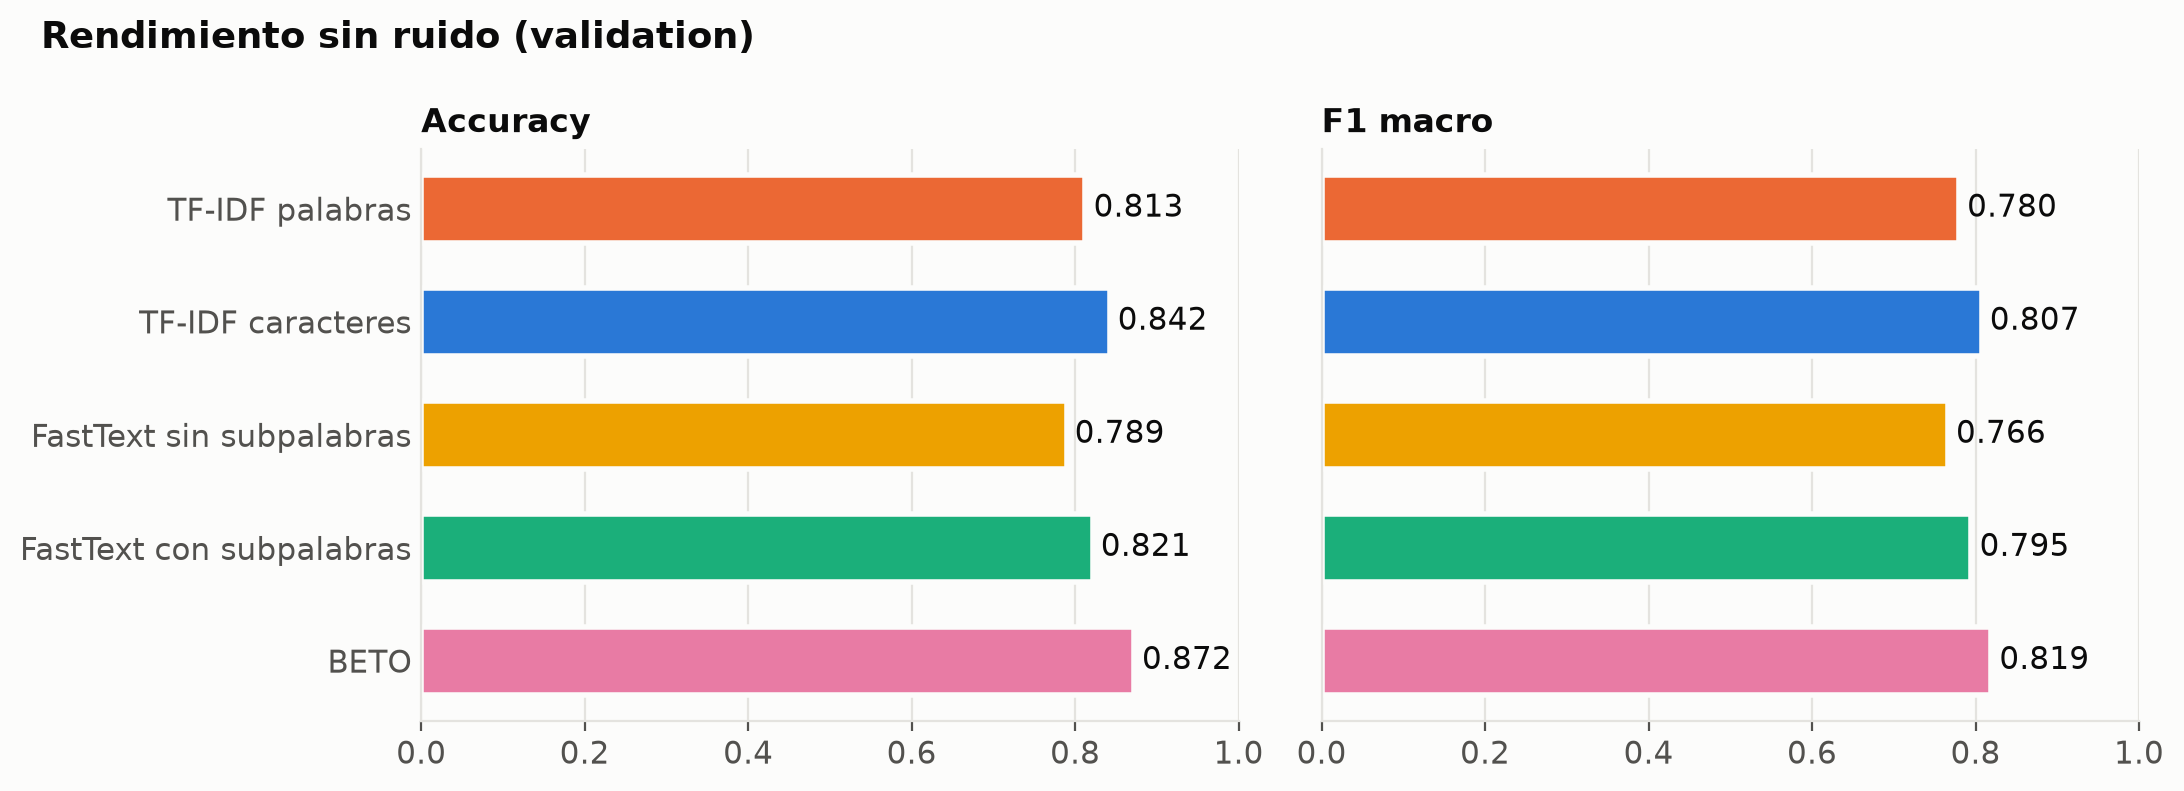
\includegraphics[width=\linewidth]{1_rendimiento_limpio.png}
\caption{Accuracy y F1 macro sin ruido sobre validation.}
\label{fig:limpio}
\end{figure}

\subsection{Degradación frente al ruido}

La Figura~\ref{fig:curvas} muestra el F1 macro según la intensidad de cada perturbación, y la
Tabla~\ref{tab:caidas} la caída de accuracy a intensidad máxima. Las perturbaciones se separan
en dos grupos muy distintos. Los errores de tipeo y el ruido combinado degradan fuertemente a
todos los modelos: con typos a $p=1{,}0$, TF-IDF de palabras pasa de un F1 macro de 0,780 a
0,074, y FastText sin subpalabras queda en un nivel similar. El resto de las perturbaciones
produce caídas pequeñas, de 0,057 puntos o menos.

\begin{figure}[H]
\centering
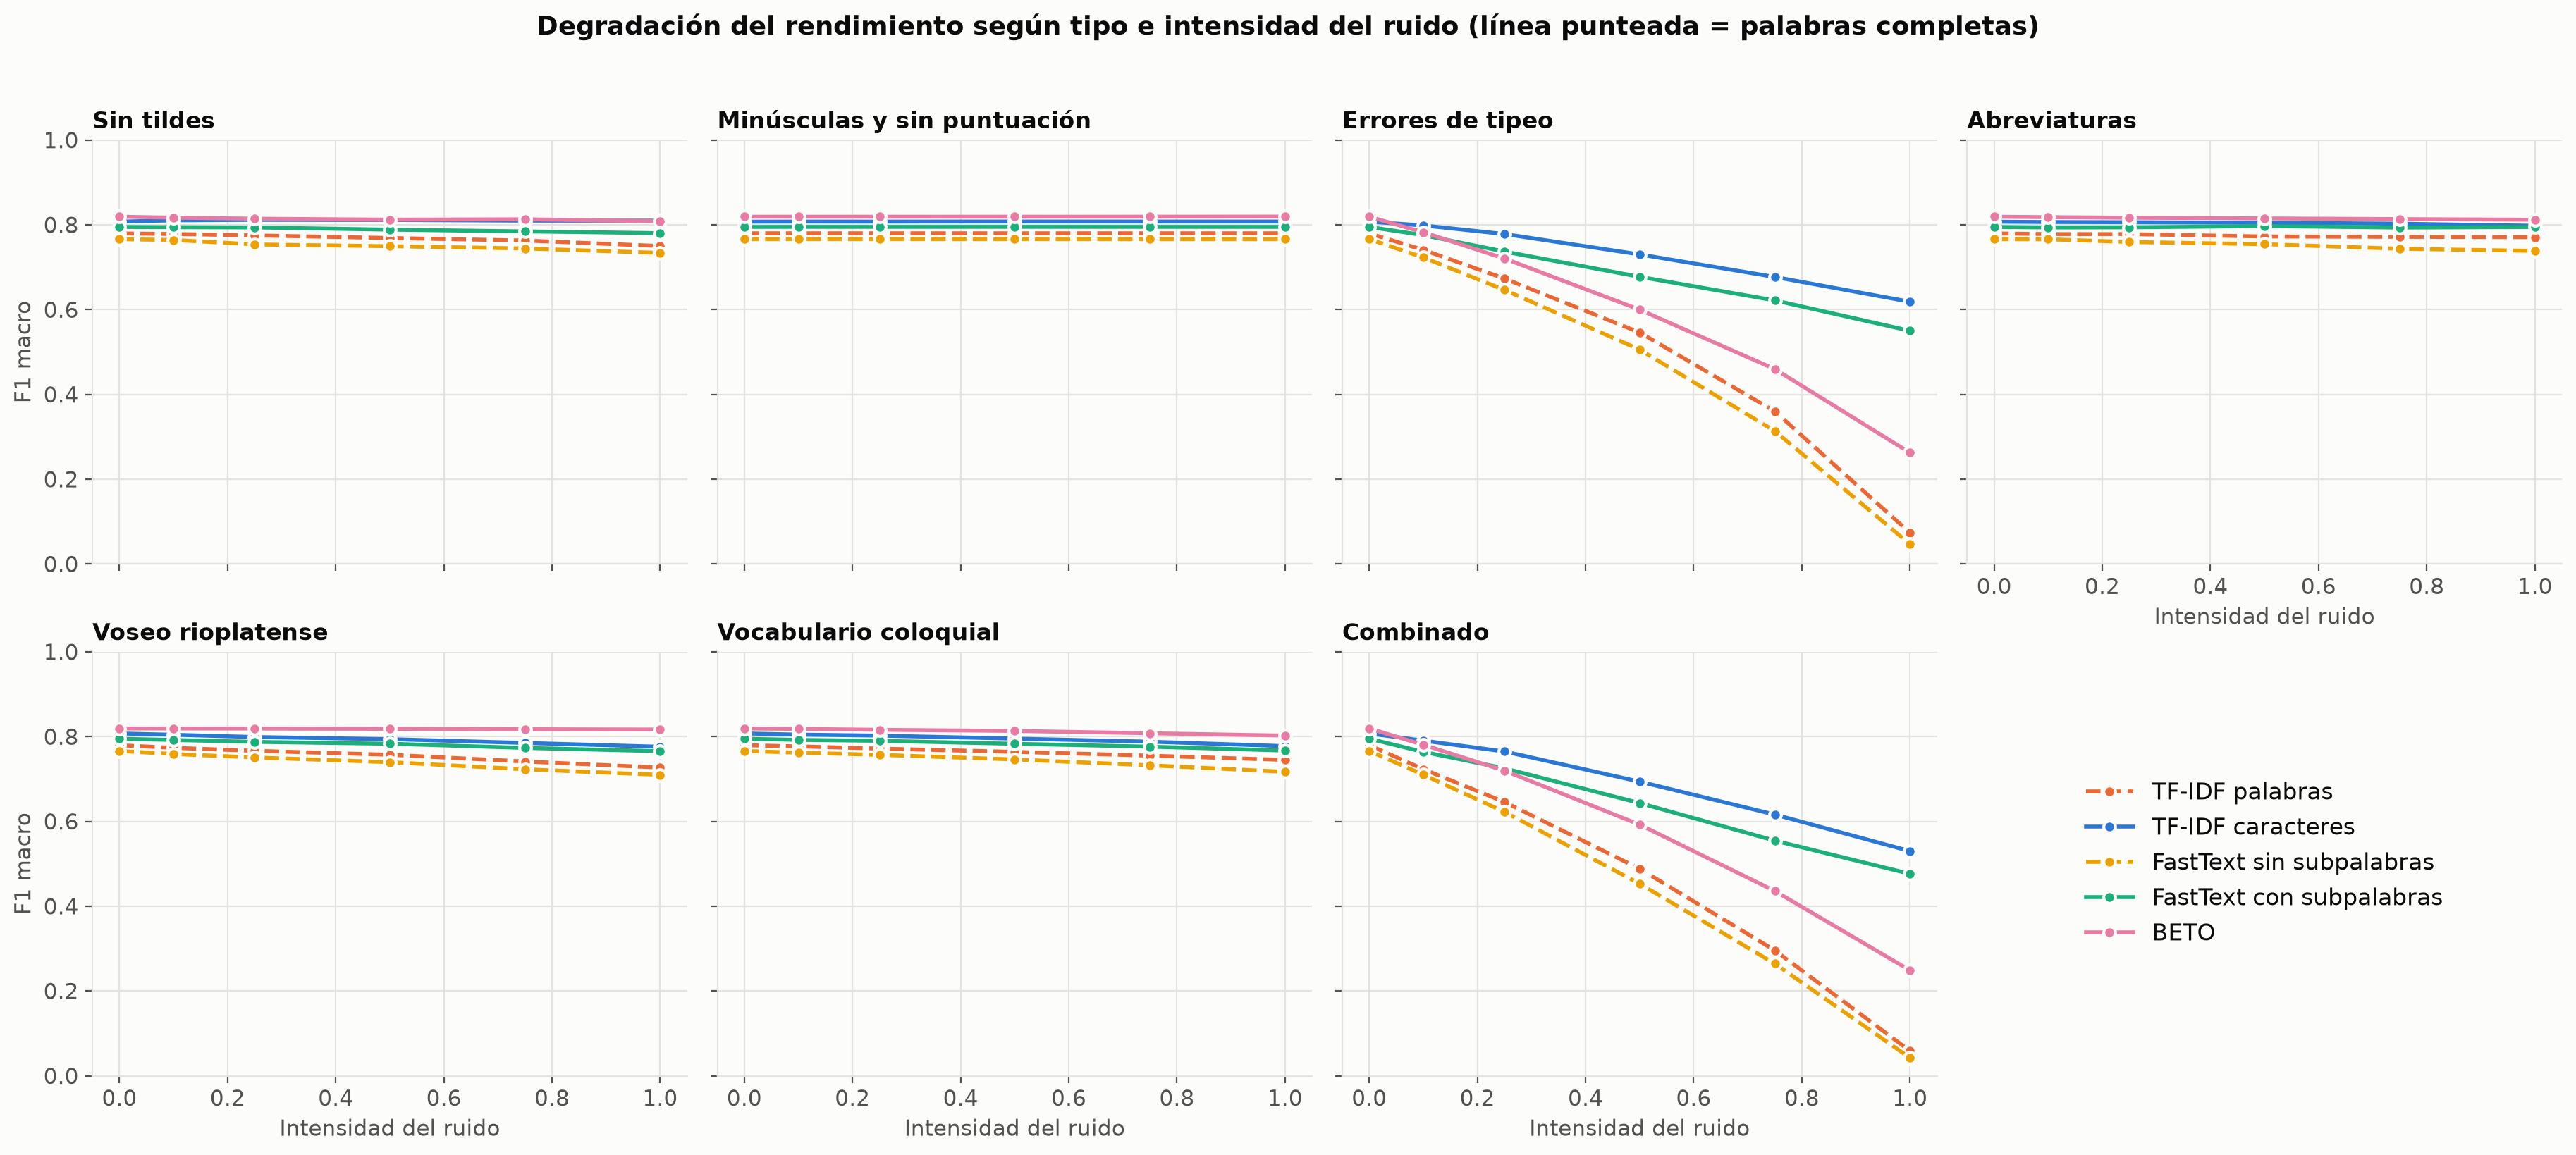
\includegraphics[width=\linewidth]{2_curvas_degradacion.png}
\caption{F1 macro según tipo e intensidad del ruido, promediado sobre semillas. Las líneas
punteadas corresponden a modelos de palabras completas.}
\label{fig:curvas}
\end{figure}

\begin{table}[H]
\centering
\small
\begin{tabular}{@{}l c c c c c@{}}
\toprule
Ruido ($p=1{,}0$) & TF-IDF pal. & TF-IDF car. & FastText sin sub. & FastText con sub. & BETO \\
\midrule
Errores de tipeo & 0,681 & \textbf{0,195} & 0,687 & 0,239 & 0,574 \\
Combinado & 0,691 & \textbf{0,303} & 0,682 & 0,333 & 0,599 \\
Vocabulario coloquial & 0,036 & 0,034 & 0,057 & 0,034 & \textbf{0,011} \\
Sin tildes & 0,033 & 0,015 & 0,031 & 0,020 & 0,014 \\
Voseo & 0,021 & 0,011 & 0,031 & 0,013 & \textbf{0,003} \\
Abreviaturas & 0,009 & 0,009 & 0,017 & 0,014 & 0,007 \\
Minúsculas y sin puntuación & 0 & 0 & 0 & 0 & 0 \\
\bottomrule
\end{tabular}
\caption{Caída de accuracy en validation (limpia menos con ruido, en puntos absolutos) a
intensidad 1,0. Menor es mejor.}
\label{tab:caidas}
\end{table}

\paragraph{Errores de tipeo: la hipótesis se confirma.} La comparación más limpia es la de
FastText con y sin subpalabras, que comparten algoritmo e hiperparámetros. La versión sin
subpalabras cae 0,448 puntos más a intensidad 1,0 (IC 95~\%: [0,426; 0,471]) y 0,067 más a
intensidad 0,25 ([0,058; 0,078]). La diferencia es significativa en todas las intensidades de
typos y de ruido combinado. TF-IDF de caracteres es el modelo más robusto, con una caída de
0,195 frente a 0,681 de TF-IDF de palabras.

\paragraph{BETO matiza la hipótesis.} Aunque BETO usa subpalabras, con typos a intensidad 1,0
pierde 0,574 puntos: mucho más que TF-IDF de caracteres (diferencia de caídas de 0,378, IC
[0,361; 0,395]), aunque menos que TF-IDF de palabras (0,107 menos, IC [0,084; 0,128]). A
intensidad 0,25 no se distingue de TF-IDF de palabras. Los dos tipos de subpalabras difieren en
cuánto se solapan las representaciones de la palabra limpia y la mal escrita: en los typos a
intensidad 1,0, el 81~\% de los pares palabra--typo no comparte \emph{ningún} token WordPiece
con la palabra original, contra el 3,9~\% que no comparte ningún n-grama de caracteres. Esto es
consistente con que lo que importa para la robustez es ese solapamiento y no el hecho de usar
subpalabras en sí, aunque se trata de una descripción y no de una prueba causal.

\paragraph{Qué ruido afecta a quién.} La Figura~\ref{fig:heatmap} resume la caída relativa del
F1 macro por modelo y perturbación, y la Figura~\ref{fig:grupos} la promedia por tipo de
representación. Separar BETO de los modelos de n-gramas de caracteres es necesario: si se los
promedia juntos, la diferencia entre ambos tipos de subpalabras queda oculta.

\begin{figure}[H]
\centering
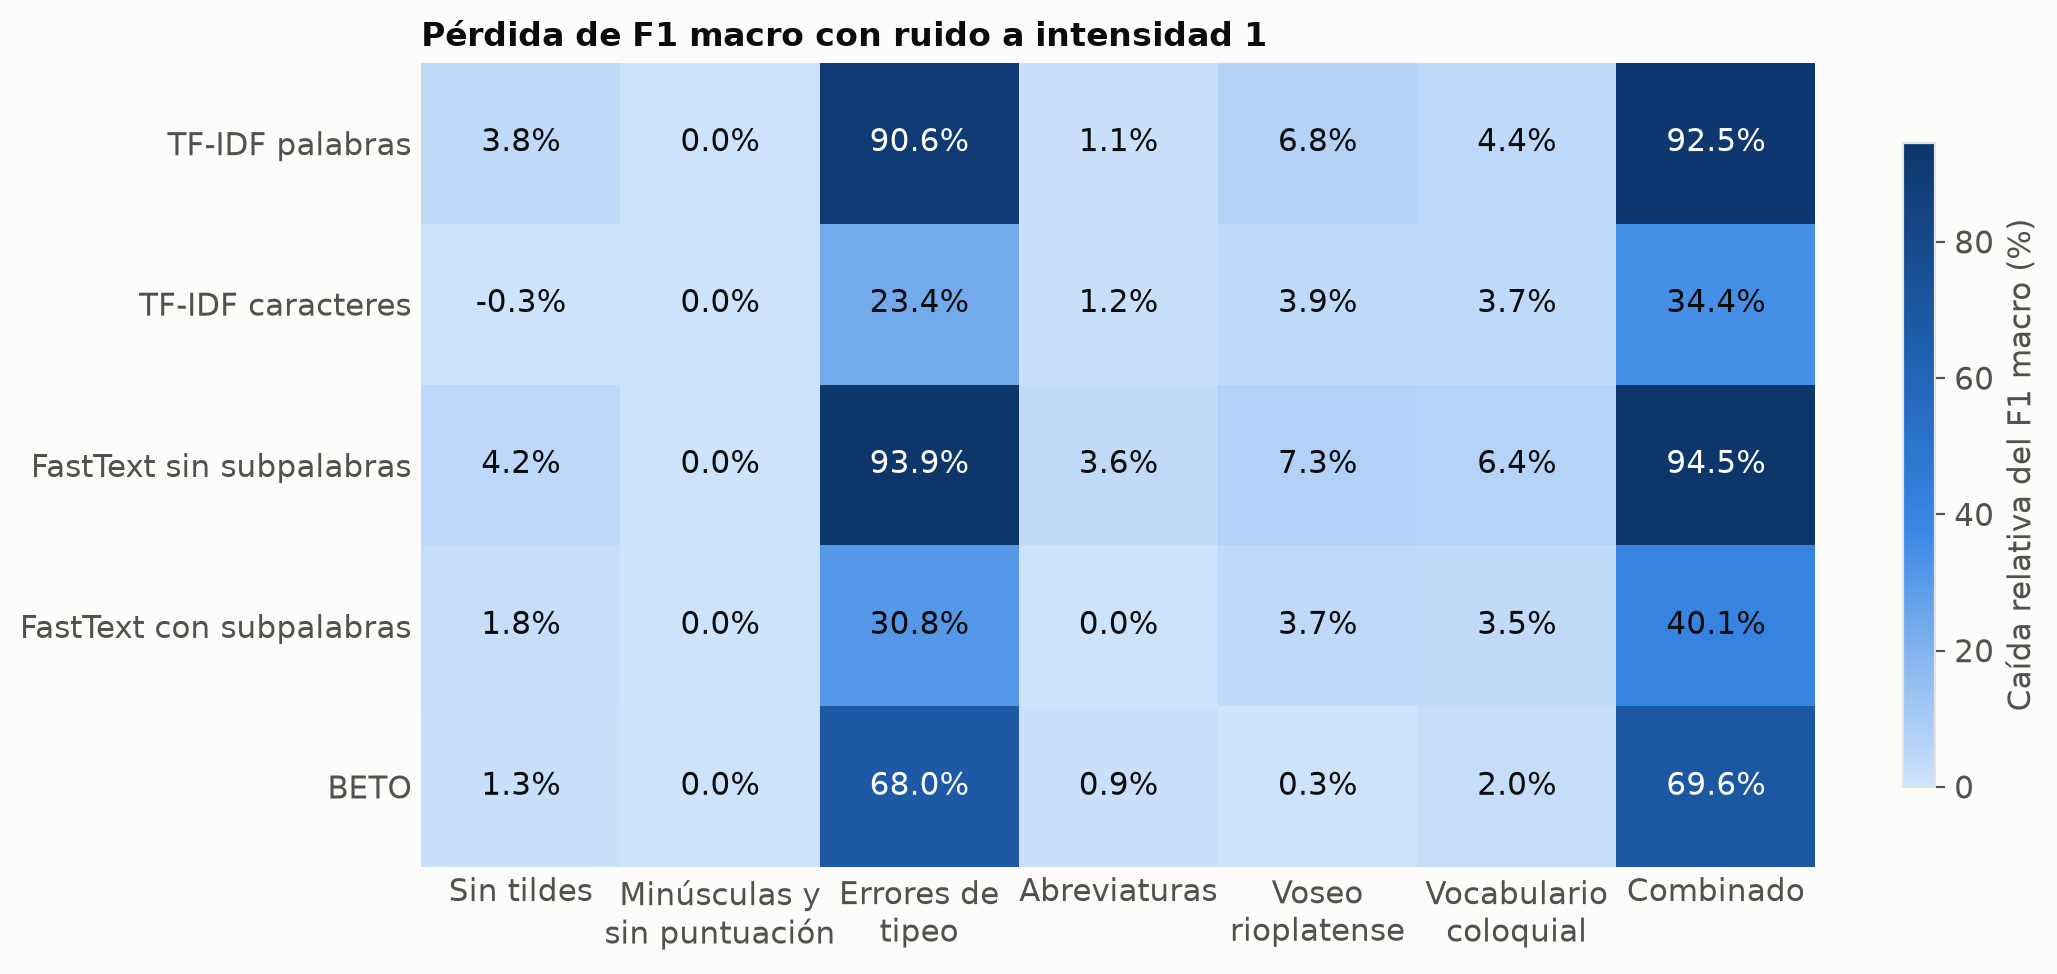
\includegraphics[width=0.85\linewidth]{3_heatmap_caida.png}
\caption{Caída relativa del F1 macro (\%) a intensidad 1,0, por modelo y perturbación.}
\label{fig:heatmap}
\end{figure}

\begin{figure}[H]
\centering
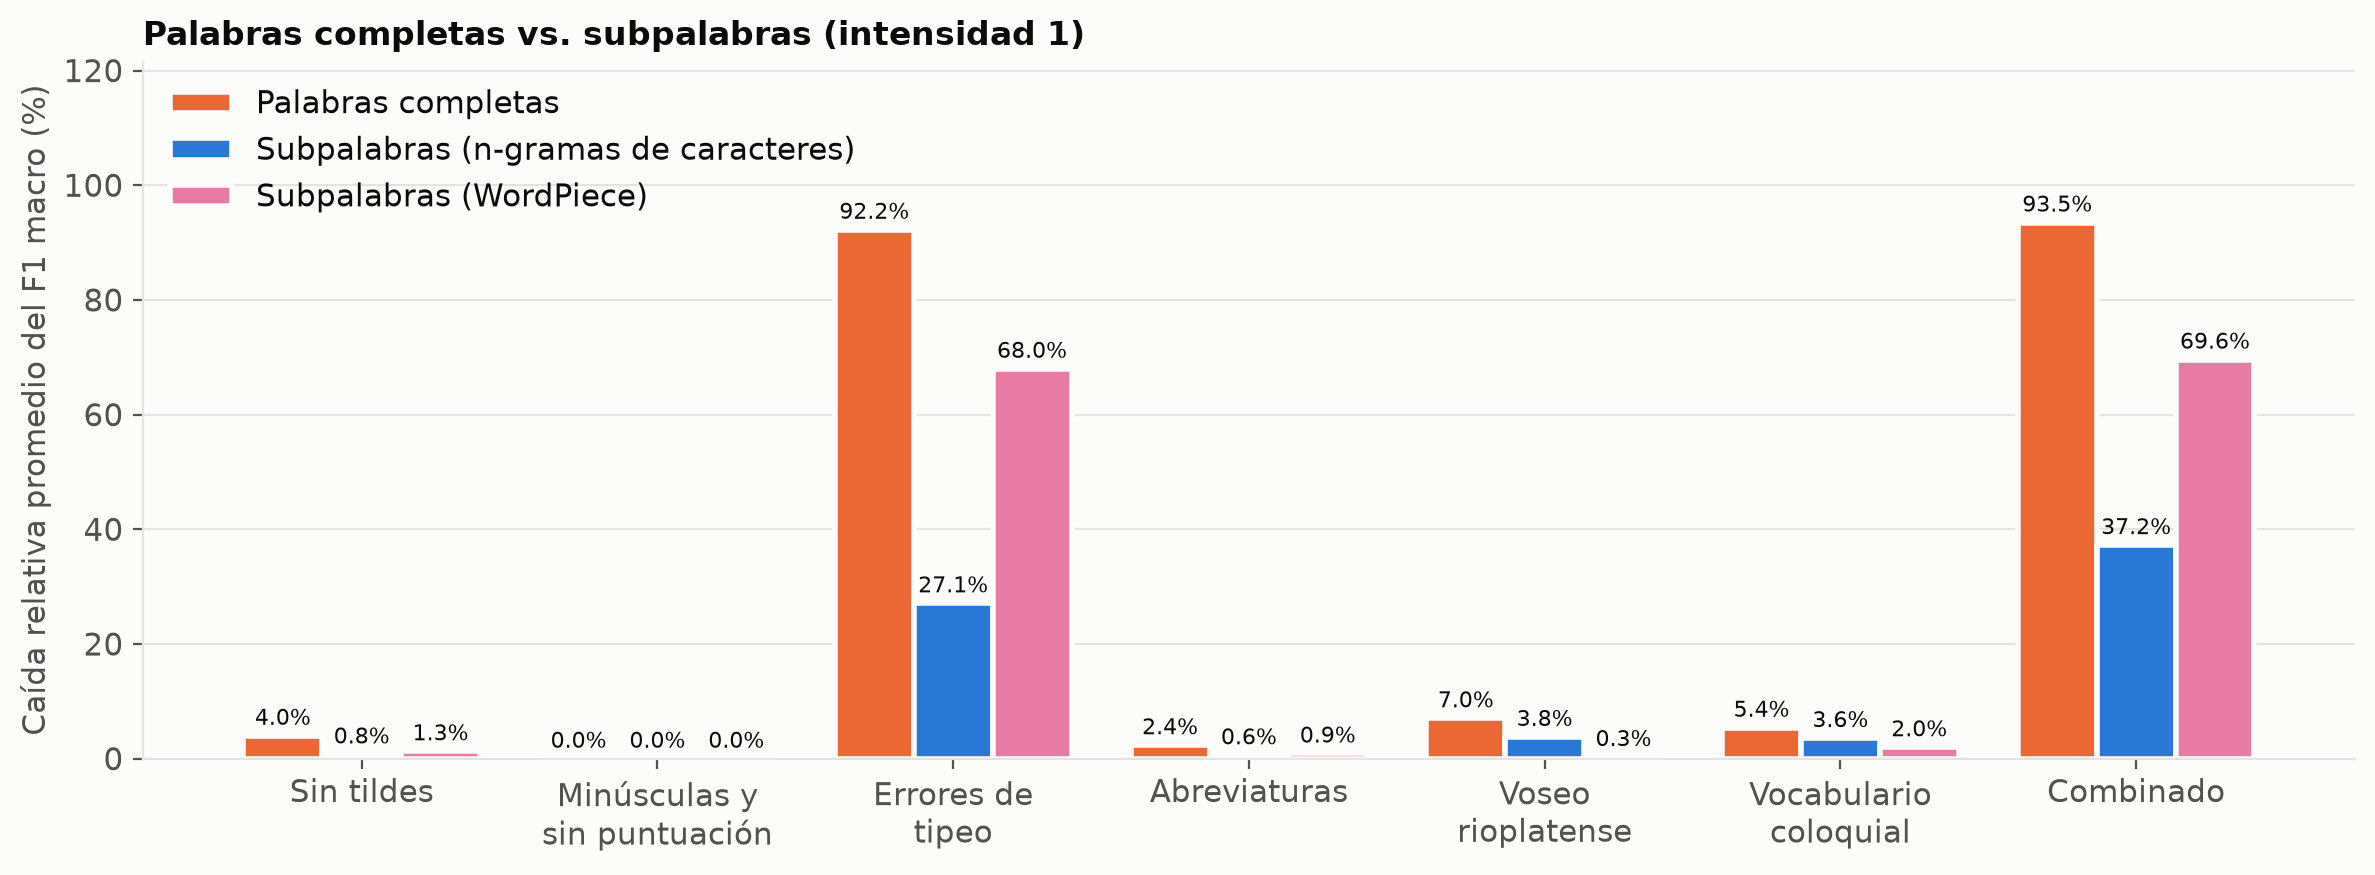
\includegraphics[width=\linewidth]{4_palabras_vs_subpalabras.png}
\caption{Caída relativa promedio del F1 macro a intensidad 1,0 por tipo de representación.}
\label{fig:grupos}
\end{figure}

\paragraph{Vocabulario coloquial y voseo.} En estos casos BETO es el más robusto (caídas de
0,011 y 0,003). En TF-IDF, palabras y caracteres no difieren ante el vocabulario coloquial
(diferencia de 0,001, IC [$-$0,007; 0,009]): \enquote{mail} no comparte n-gramas con
\enquote{correo}, así que es un problema de vocabulario que las subpalabras no pueden
compensar. En FastText la diferencia existe pero es chica (0,023, IC [0,013; 0,034]).
Es plausible que el preentrenamiento de BETO sobre un corpus amplio incluya estas variantes,
aunque no se verificó.

\paragraph{Tildes, abreviaturas, minúsculas.} El efecto de quitar tildes es pequeño en todos
los modelos ($\leq$ 0,033) y no se puede afirmar que BETO supere a TF-IDF de caracteres
(diferencia de 0,001, IC [$-$0,008; 0,011]). Las abreviaturas tienen un efecto de 0,017 o
menos, sin diferencias significativas entre modelos. La perturbación de minúsculas y
puntuación no tiene efecto, porque MASSIVE ya viene en minúsculas y casi sin puntuación.

\subsection{Comparación con LLM locales}
\label{sec:llm}

La Tabla~\ref{tab:llm} y la Figura~\ref{fig:llm} comparan los LLM con los modelos entrenados.
Ningún LLM supera a TF-IDF de caracteres en ninguna condición: con typos a intensidad 1,0,
el mejor LLM, \cod{qwen3.5:4b}, obtiene 0,554 contra 0,647. Tampoco superan a FastText con
subpalabras, salvo un empate con ruido combinado a intensidad 1,0. Contra BETO sí hay un
cruce: BETO empieza muy por encima pero termina por debajo de ambos LLM con typos intensos
(diferencia de caídas con \cod{qwen3.5:4b} de 0,398, IC [0,373; 0,423]); el cruce se observa
en la figura pero no se calculó con un intervalo de confianza.

En cuanto a la robustez, \cod{qwen3.5:4b} con $k=2$ cae ante typos casi lo mismo que TF-IDF de
caracteres (diferencia de $-$0,020, IC [$-$0,042; 0,002]), mientras que con $k=0$ cae más
(0,049, IC [0,025; 0,074]). Sin ruido, $k=0$ y $k=2$ rinden casi igual (0,725 y 0,730): los
ejemplos del prompt ayudan más a la robustez que al nivel base.

El costo es mucho mayor. La latencia mediana de los LLM es unas mil veces la de TF-IDF de
caracteres y unas noventa veces la de BETO. Por cada mil frases, la GPU consume 0,017~Wh con
BETO, 12,7~Wh con \cod{llama3.1} y 21,0~Wh con \cod{qwen3.5:4b}. TF-IDF y FastText corren en
CPU, y la medición de la GPU no los representa. \cod{qwen3.5:4b} resultó más lento y de mayor
consumo que \cod{llama3.1} pese a ser más chico; no se investigó la causa. Para esta tarea,
entonces, el costo energético de los modelos grandes
no se traduce en una mejora de robustez.

\begin{table}[H]
\centering
\small
\begin{tabular}{@{}l c c c r r@{}}
\toprule
Modelo & Limpio & Typos 1,0 & Combinado 1,0 & p50 (ms) & Frases/s \\
\midrule
TF-IDF caracteres & 0,842 & \textbf{0,647} & \textbf{0,539} & 0,54 & 26\,373 \\
FastText con subpalabras & 0,821 & 0,582 & 0,489 & 0,012 & 33\,974 \\
BETO & \textbf{0,872} & 0,298 & 0,273 & 6,25 & 3\,047 \\
\cod{llama3.1} ($k=2$) & 0,670 & 0,470 & 0,412 & 569 & 7,0 \\
\cod{qwen3.5:4b} ($k=2$) & 0,730 & 0,554 & 0,494 & 1\,062 & 3,8 \\
\bottomrule
\end{tabular}
\caption{Accuracy en validation y costo de inferencia. p50: latencia mediana al clasificar una
frase por vez. Frases/s: rendimiento al clasificar el conjunto completo.}
\label{tab:llm}
\end{table}

\begin{figure}[H]
\centering
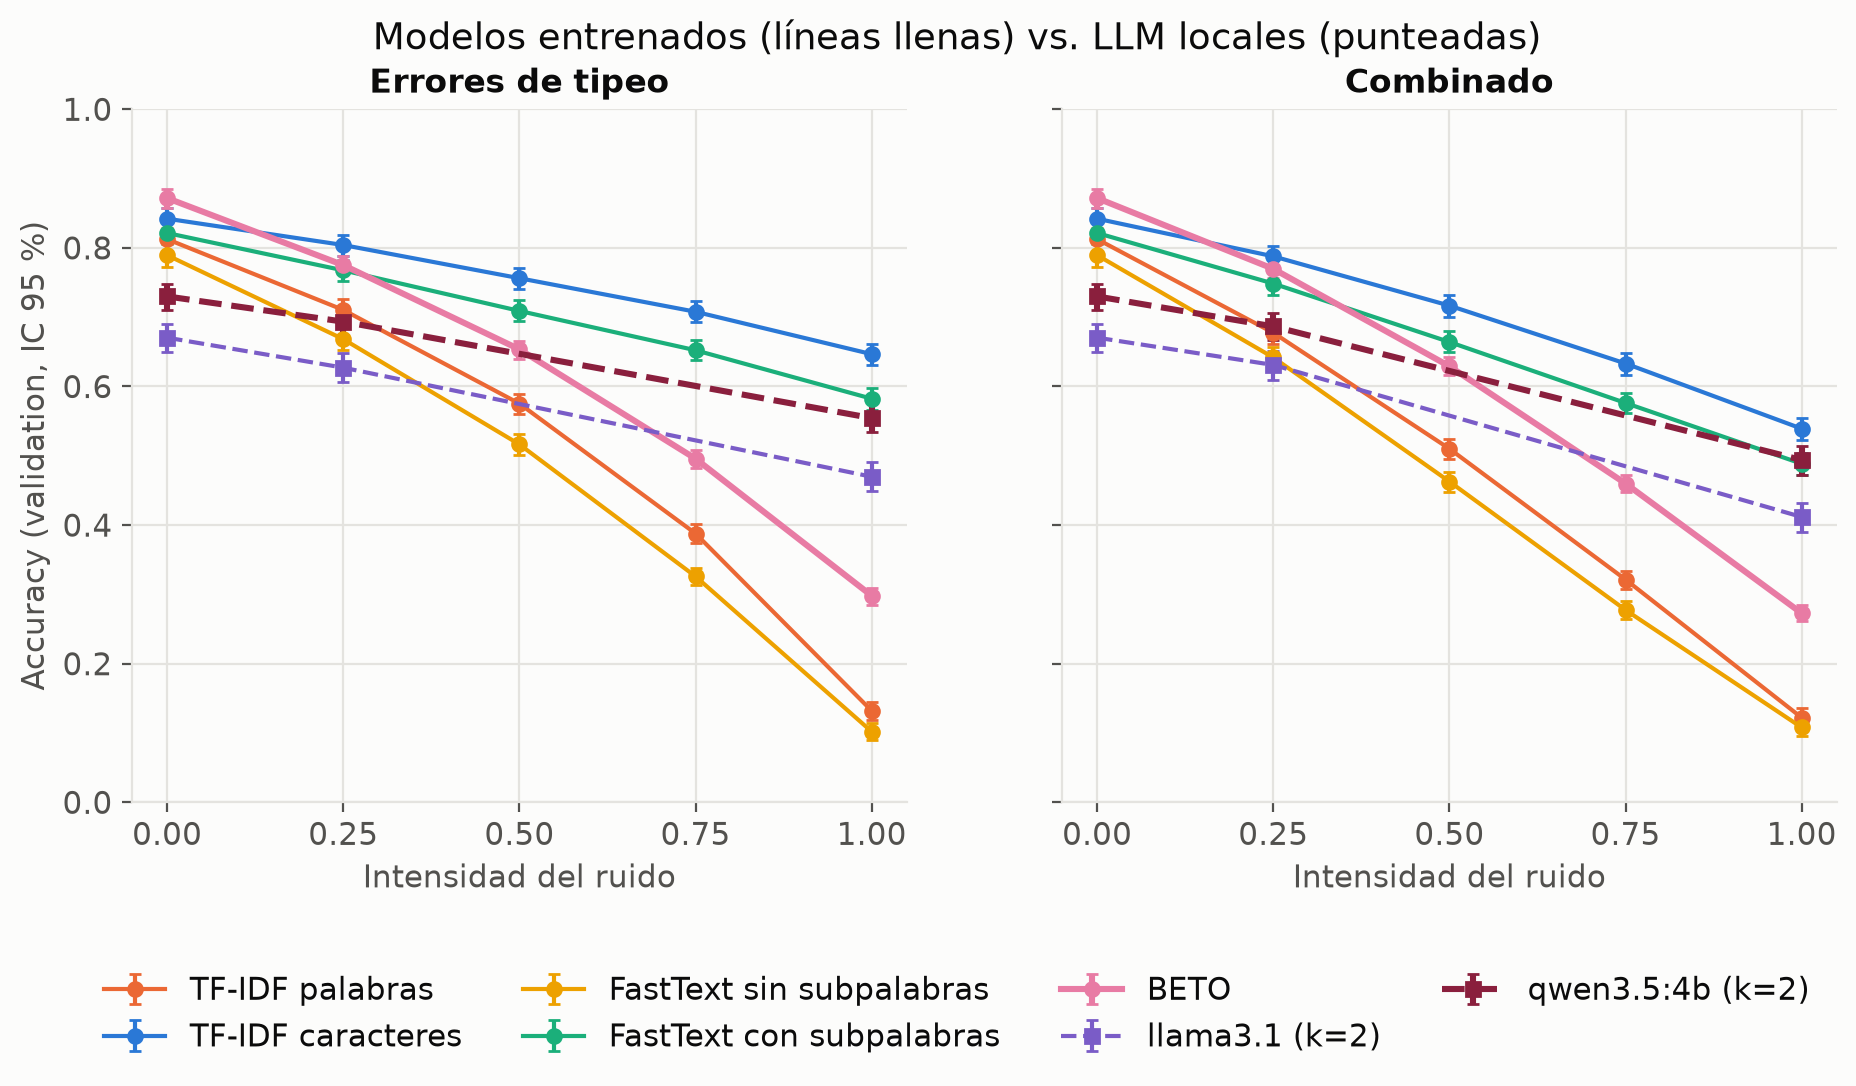
\includegraphics[width=0.64\linewidth]{6_cruce_llm.png}
\caption{Accuracy (IC 95~\%) según la intensidad de los typos y del ruido combinado. Los LLM
solo se evaluaron a intensidad 0,25 y 1,0.}
\label{fig:llm}
\end{figure}

% ---------------------------------------------------------------------------
\section{Discusión, análisis de errores y limitaciones}

\subsection{Análisis de errores}

\paragraph{Confusión de base.} Sin ruido, los errores se concentran en pares de intenciones
semánticamente cercanas: en promedio entre modelos, el 33~\% de las frases de
\cod{music\_settings} se clasifica como \cod{play\_music}, el 24~\% de
\cod{datetime\_convert} como \cod{datetime\_query} y alrededor del 21~\% de \cod{qa\_maths} como
\cod{qa\_factoid}. La intención \cod{general\_quirky}, que agrupa frases variadas, funciona
como sumidero de errores. Con ruido el fenómeno se acentúa: cuando TF-IDF de palabras no
reconoce las palabras de la frase, la predicción tiende a \cod{general\_quirky}, que es la
confusión más frecuente con ruido combinado a intensidad 0,5.

\paragraph{Dónde ganan los n-gramas de caracteres.} Con typos a intensidad 0,5, hay 438
frases en las que TF-IDF de caracteres acierta y TF-IDF de palabras falla, contra 76 en el
sentido contrario. Un ejemplo típico es \enquote{puedes crrear uha nueca listta}
(\cod{lists\_createoradd}): las tres palabras con typo son desconocidas para el modelo de
palabras, que predice \cod{general\_quirky}, mientras que los n-gramas de caracteres conservan
suficientes fragmentos para acertar. En los casos inversos, el typo suele producir fragmentos
que se parecen a otra intención: \enquote{avísame a las cino hora} se clasifica como
\cod{calendar\_set} en lugar de \cod{alarm\_set}.

\paragraph{Intenciones más afectadas.} La Figura~\ref{fig:intenciones} muestra las diez
intenciones que más F1 pierde TF-IDF de palabras con ruido combinado a intensidad 0,5. En
todas ellas TF-IDF de caracteres pierde bastante menos. Las más afectadas dependen de pocas
palabras clave (\cod{iot\_wemo\_on}, \cod{audio\_volume\_down}, \cod{alarm\_remove}), y
basta con alterar esas palabras para que el modelo de palabras se quede sin evidencia.

\begin{figure}[H]
\centering
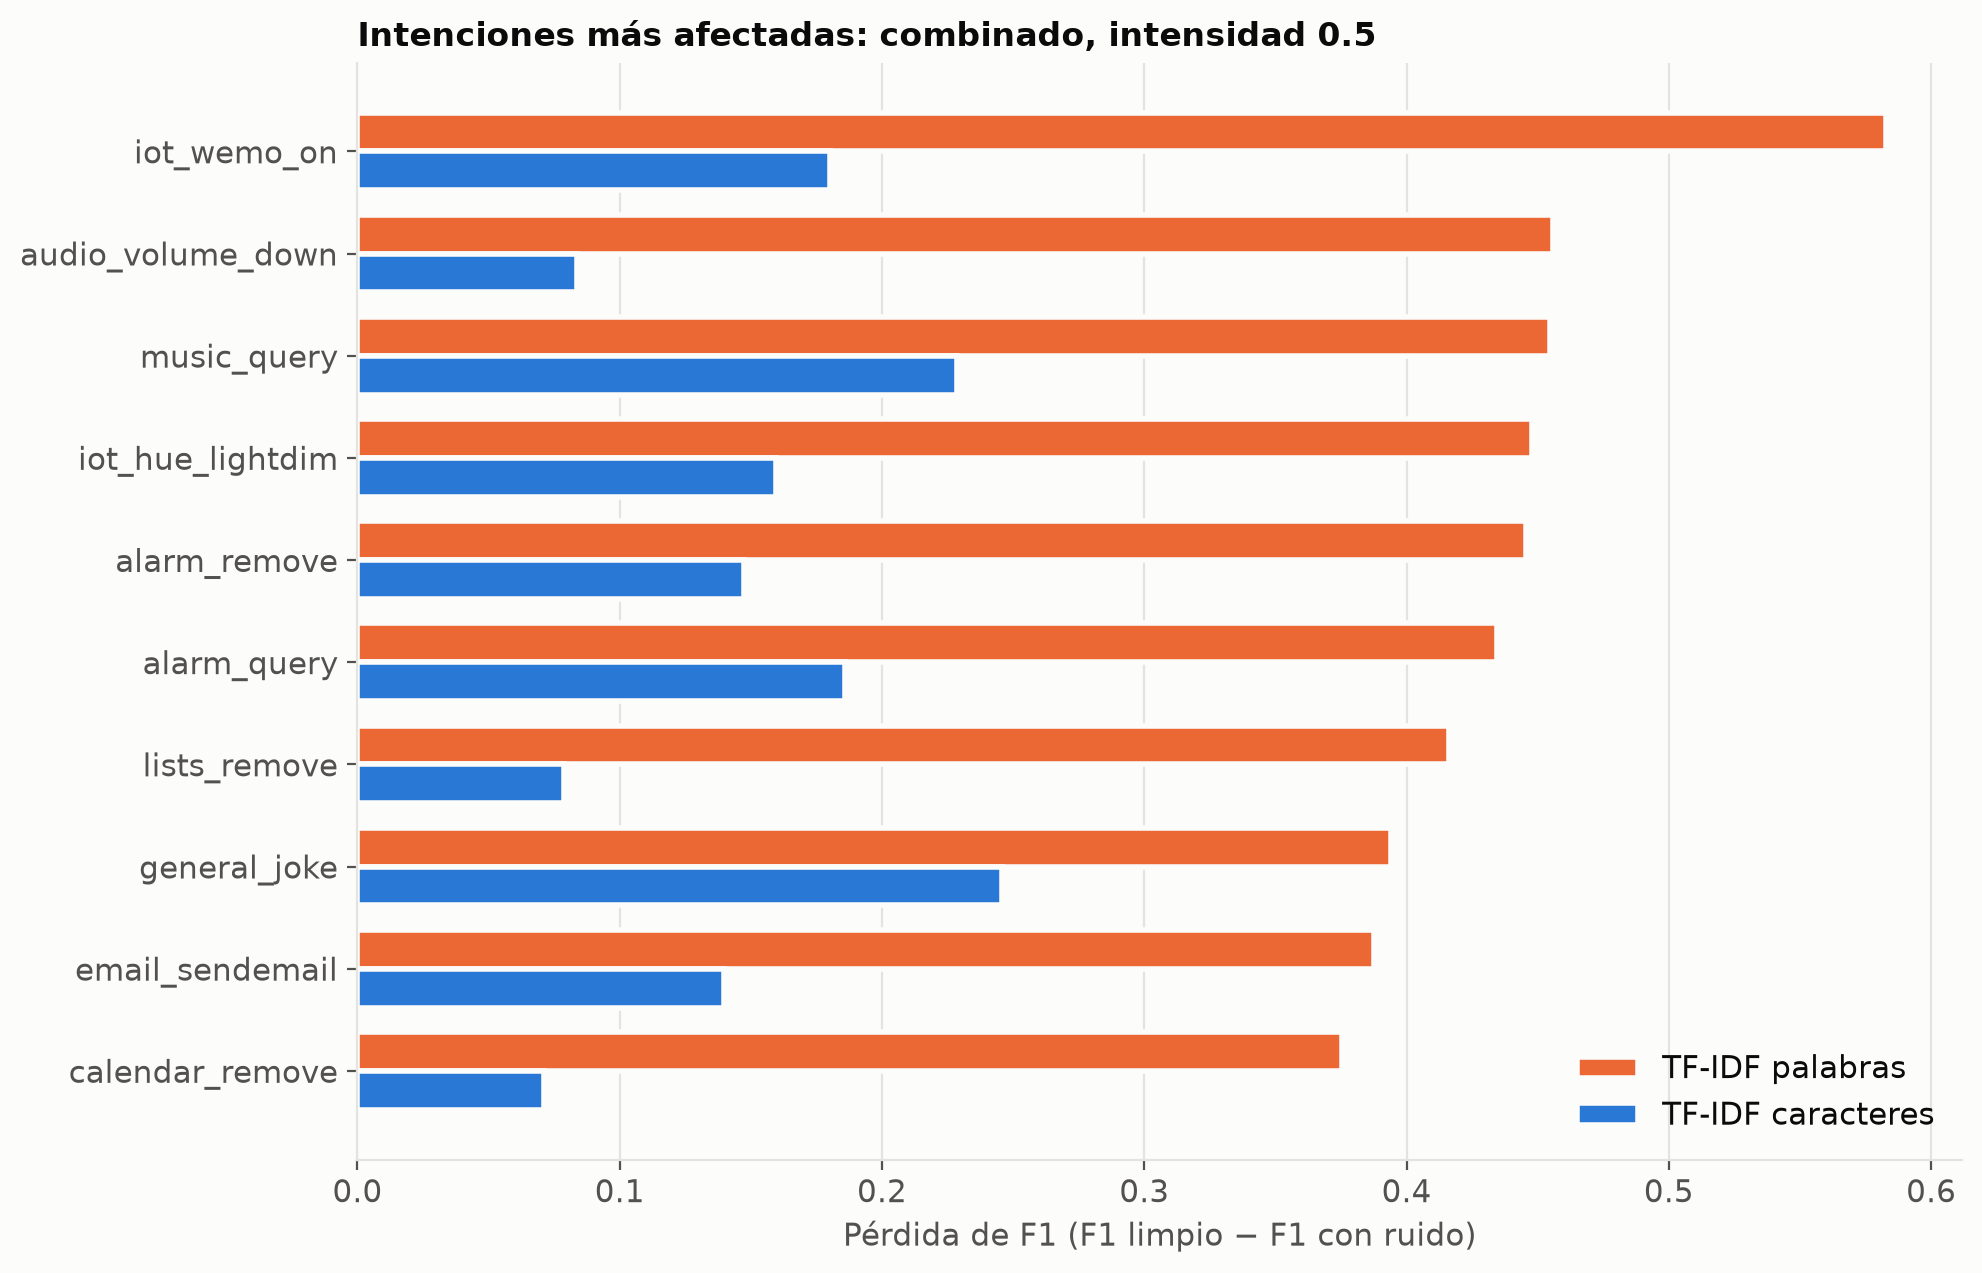
\includegraphics[width=0.8\linewidth]{5_intenciones_afectadas.png}
\caption{Intenciones con mayor pérdida de F1 para TF-IDF de palabras con ruido combinado a
intensidad 0,5, comparadas con TF-IDF de caracteres.}
\label{fig:intenciones}
\end{figure}

\paragraph{Abreviaturas y modelos de palabras.} De las abreviaturas usadas, solo
\enquote{cumple} aparece en el vocabulario de entrenamiento. Un modelo TF-IDF ignora los tokens
desconocidos, así que para TF-IDF de palabras abreviar equivale a borrar la palabra. Que la
caída sea pequeña indica que las palabras abreviadas (\enquote{de}, \enquote{que},
\enquote{por}, \enquote{para}) aportan poca información sobre la intención, no que el modelo
entienda las abreviaturas.

\subsection{Limitaciones}

\begin{itemize}
  \item \textbf{Ruido sintético.} Las perturbaciones aproximan, pero no reproducen, los errores
        reales de los usuarios. La intensidad 1,0 de typos (un error en cada palabra de tres o
        más letras) es extrema y sirve como cota más que como escenario realista.
  \item \textbf{Diccionarios hechos a mano.} Los diccionarios de abreviaturas, voseo y
        vocabulario coloquial son chicos, tienen sesgo rioplatense y se aplican sobre un
        corpus de español de España. Algunos reemplazos son aproximados (\enquote{taxi}
        $\to$ \enquote{remis}, \enquote{reunión} $\to$ \enquote{junta}).
  \item \textbf{Perturbación sin efecto.} Como MASSIVE ya viene en minúsculas y casi sin
        puntuación, la perturbación correspondiente no pudo evaluarse.
  \item \textbf{Tamaño de la evaluación.} La robustez se mide sobre 2\,033 frases, y algunas
        intenciones tienen cinco frases o menos, por lo que su F1 es inestable.
  \item \textbf{Comparaciones múltiples.} Se calcularon 56 comparaciones con intervalos del
        95~\%; es esperable que unas tres excluyan el cero por azar. Las conclusiones
        principales se apoyan en diferencias muy por encima de ese umbral.
  \item \textbf{Variabilidad.} Los intervalos de confianza reflejan la muestra de frases, no la
        variabilidad entre semillas de entrenamiento. TF-IDF se entrenó con una sola semilla.
        FastText no es reproducible de forma exacta entre plataformas (por ejemplo, 0,807 de
        accuracy en test en Linux y 0,805 en macOS).
  \item \textbf{Comparación con LLM.} Se probaron dos modelos con un prompt cada uno, con una
        semilla de ruido y dos intensidades. La latencia de los LLM incluye el servidor y la
        comunicación HTTP, con cuatro pedidos en paralelo, mientras que la de los demás
        modelos se mide dentro del mismo proceso, por lo que la comparación solo es válida en
        orden de magnitud.
  \item \textbf{Sin entrenamiento con ruido.} No se evaluó si entrenar con datos aumentados con
        ruido permite a los modelos de palabras recuperar robustez.
\end{itemize}

% ---------------------------------------------------------------------------
\section{Conclusiones}

Se construyeron y compararon cinco clasificadores de intenciones en español sobre MASSIVE, y se
midió su degradación frente a siete tipos de ruido de escritura con intensidad controlada y
con intervalos de confianza.

La hipótesis se \textbf{confirma para los errores de tipeo en los modelos de n-gramas de
caracteres}. El control experimental de FastText, en el que solo cambia el uso de subpalabras,
muestra una diferencia de caída de 0,448 puntos de accuracy a intensidad máxima, y TF-IDF de
caracteres es el modelo más robusto en todas las intensidades de typos y de ruido combinado.

La hipótesis \textbf{no se cumple de forma general para todos los tokenizadores de
subpalabras}. BETO es el mejor modelo sin ruido, pero ante typos intensos cae casi tanto como
los modelos de palabras completas. Su vocabulario WordPiece fijo hace que la palabra mal
escrita casi nunca comparta tokens con la original, mientras que los n-gramas de caracteres
casi siempre comparten alguno. Lo que parece importar no es solo usar subpalabras, sino cuánto
se solapan las representaciones de la forma correcta y la errónea.

Respecto de la pregunta complementaria, la diferencia entre representaciones se manifiesta
casi exclusivamente en los errores de tipeo y en el ruido combinado que los incluye. Ante
cambios de vocabulario y voseo las caídas son pequeñas, y allí el mejor es BETO, posiblemente
por su preentrenamiento. Quitar tildes y abreviar tiene poco efecto sobre todos los modelos.

En la práctica, para un asistente que recibe texto informal, un modelo liviano como TF-IDF de
caracteres ofrece el mejor equilibrio entre robustez a typos y costo, y un transformer como
BETO convendría combinarlo con corrección ortográfica o con entrenamiento sobre datos con
ruido. Los LLM locales evaluados no aportaron mayor robustez que los n-gramas de caracteres y
resultaron unas mil veces más lentos.

Como trabajo futuro queda entrenar con datos aumentados con ruido, evaluar con errores reales
de usuarios y probar otros transformers, por ejemplo multilingües o con tokenización a nivel
de caracteres.

\nocite{*}
\printbibliography[title={Bibliografía}]

\end{document}
